
%% bare_jrnl_compsoc.tex
%% V1.4b
%% 2015/08/26
%% by Michael Shell
%% See:
%% http://www.michaelshell.org/
%% for current contact information.
%%
%% This is a skeleton file demonstrating the use of IEEEtran.cls
%% (requires IEEEtran.cls version 1.8b or later) with an IEEE
%% Computer Society journal paper.
%%
%% Support sites:
%% http://www.michaelshell.org/tex/ieeetran/
%% http://www.ctan.org/pkg/ieeetran
%% and
%% http://www.ieee.org/

%%*************************************************************************
%% Legal Notice:
%% This code is offered as-is without any warranty either expressed or
%% implied; without even the implied warranty of MERCHANTABILITY or
%% FITNESS FOR A PARTICULAR PURPOSE!
%% User assumes all risk.
%% In no event shall the IEEE or any contributor to this code be liable for
%% any damages or losses, including, but not limited to, incidental,
%% consequential, or any other damages, resulting from the use or misuse
%% of any information contained here.
%%
%% All comments are the opinions of their respective authors and are not
%% necessarily endorsed by the IEEE.
%%
%% This work is distributed under the LaTeX Project Public License (LPPL)
%% ( http://www.latex-project.org/ ) version 1.3, and may be freely used,
%% distributed and modified. A copy of the LPPL, version 1.3, is included
%% in the base LaTeX documentation of all distributions of LaTeX released
%% 2003/12/01 or later.
%% Retain all contribution notices and credits.
%% ** Modified files should be clearly indicated as such, including  **
%% ** renaming them and changing author support contact information. **
%%*************************************************************************


% *** Authors should verify (and, if needed, correct) their LaTeX system  ***
% *** with the testflow diagnostic prior to trusting their LaTeX platform ***
% *** with production work. The IEEE's font choices and paper sizes can   ***
% *** trigger bugs that do not appear when using other class files.       ***                          ***
% The testflow support page is at:
% http://www.michaelshell.org/tex/testflow/


\documentclass[10pt,journal,compsoc]{IEEEtran}
%
% If IEEEtran.cls has not been installed into the LaTeX system files,
% manually specify the path to it like:
% \documentclass[10pt,journal,compsoc]{../sty/IEEEtran}





% Some very useful LaTeX packages include:
% (uncomment the ones you want to load)


% *** MISC UTILITY PACKAGES ***
%
%\usepackage{ifpdf}
% Heiko Oberdiek's ifpdf.sty is very useful if you need conditional
% compilation based on whether the output is pdf or dvi.
% usage:
% \ifpdf
%   % pdf code
% \else
%   % dvi code
% \fi
% The latest version of ifpdf.sty can be obtained from:
% http://www.ctan.org/pkg/ifpdf
% Also, note that IEEEtran.cls V1.7 and later provides a builtin
% \ifCLASSINFOpdf conditional that works the same way.
% When switching from latex to pdflatex and vice-versa, the compiler may
% have to be run twice to clear warning/error messages.






% *** CITATION PACKAGES ***
%
\ifCLASSOPTIONcompsoc
  % IEEE Computer Society needs nocompress option
  % requires cite.sty v4.0 or later (November 2003)
  \usepackage[nocompress]{cite}
\else
  % normal IEEE
  \usepackage{cite}
\fi





% *** GRAPHICS RELATED PACKAGES ***
%
\ifCLASSINFOpdf
  % \usepackage[pdftex]{graphicx}
  % declare the path(s) where your graphic files are
  % \graphicspath{{../pdf/}{../jpeg/}}
  % and their extensions so you won't have to specify these with
  % every instance of \includegraphics
  % \DeclareGraphicsExtensions{.pdf,.jpeg,.png}
\else
  % or other class option (dvipsone, dvipdf, if not using dvips). graphicx
  % will default to the driver specified in the system graphics.cfg if no
  % driver is specified.
  % \usepackage[dvips]{graphicx}
  % declare the path(s) where your graphic files are
  % \graphicspath{{../eps/}}
  % and their extensions so you won't have to specify these with
  % every instance of \includegraphics
  % \DeclareGraphicsExtensions{.eps}
\fi
% graphicx was written by David Carlisle and Sebastian Rahtz. It is
% required if you want graphics, photos, etc. graphicx.sty is already
% installed on most LaTeX systems. The latest version and documentation
% can be obtained at:
% http://www.ctan.org/pkg/graphicx
% Another good source of documentation is "Using Imported Graphics in
% LaTeX2e" by Keith Reckdahl which can be found at:
% http://www.ctan.org/pkg/epslatex
%
% latex, and pdflatex in dvi mode, support graphics in encapsulated
% postscript (.eps) format. pdflatex in pdf mode supports graphics
% in .pdf, .jpeg, .png and .mps (metapost) formats. Users should ensure
% that all non-photo figures use a vector format (.eps, .pdf, .mps) and
% not a bitmapped formats (.jpeg, .png). The IEEE frowns on bitmapped formats
% which can result in "jaggedy"/blurry rendering of lines and letters as
% well as large increases in file sizes.
%
% You can find documentation about the pdfTeX application at:
% http://www.tug.org/applications/pdftex




\hyphenation{op-tical net-works semi-conduc-tor}
% simple interligne demandé par Mr Chaumette
\usepackage{setspace}
\singlespacing

\usepackage{graphicx}
\usepackage{textcomp}
\usepackage[table]{xcolor}
\begin{document}
%
% paper title
% Titles are generally capitalized except for words such as a, an, and, as,
% at, but, by, for, in, nor, of, on, or, the, to and up, which are usually
% not capitalized unless they are the first or last word of the title.
% Linebreaks \\ can be used within to get better formatting as desired.
% Do not put math or special symbols in the title.
\title{Tethys's report : Collecting Sensor Data Without Infrastructure or Trust}

\author{Carlos NEZOUT,
        Serigne Amsatou SEYE}% <-this % stops a space}

\IEEEtitleabstractindextext{%
% Note that keywords are not normally used for peerreview papers.
\begin{IEEEkeywords}
Internet of Things, Wireless Sensor Networks, Crowdsourcing, Energy Harvesting\ldots
\end{IEEEkeywords}}


% make the title area
\maketitle


\IEEEdisplaynontitleabstractindextext
\IEEEpeerreviewmaketitle

% https://docs.google.com/document/d/1bLFr8j81hDXjz_uRY9hrLy7u50bS6_LtlFJ-n4pVzD0/edit?usp=sharing

\section{Introduction}\label{sec:introduction}
The purpose of this report is to summarize a document published during 2018 IEEE/ACM Third International Conference on Internet-of-Things Design and Implementation. It's about Tethys, a system collecting sensor data without infrastructure. This paper will allow us to clear subjectively the relevance or not of this report.

First of all, we will contextualize the paper and present some related works raising existing approach on some meanfull terms of that subject. Then we'll clear goals of the paper, explain their contribution and some reviews before concluding.
\section{Context and Related Work}\label{sec:context}
\subsection{Context}
At the time of digital transformation, all innovative technologies are connected. Analysis and exploitation of the digital data that results from these devices provides axes of study to improve daily habits. In this case, this paper focuses on the consumption of water in residential buildings using Tethys. It's a "\emph{wireless water flow sensor that collects data at perfixture granularity without dependence on existing infrastructure and trusted gateways}"\cite{IEEEhowto:}. From a physical point of view, Tethys strongly decouples the energy dependence of the device to the infrastructure where it is deployed. It uses the water flow to mainly feed the proper functioning of its system and thus prevents any failures not correlated to infrastructure. Tethys uses crowdsourcing to collect all related data from residential consumers such as students. This process can present some inconvenient cause they can trust on consumer's phone reliability, so they need to enforce security between the sensing device and backend system ("\emph{reliability end-to-end}").

The first results they obtained show that this device is able to identify significant behaviors in the shower use. They placed about several sensors and collected data during 2 weeks. The analysis of these data makes it possible to sensitize a consumer punctually on his water consumption. This approach revealed a significant variation in average water consumption for a shower.

\subsection{Related Work}
---------------------------------------------------------------- 
//Voir partie VII. //
\section{Paper Goals}\label{sec:paperGoals}

Existing measurement models for building-wide consumption do not reveal specific information at scale of a resident. Indeed, as the Motivation's Content of the document shows us, we can know what was the daily consumption of a building, but these data are not subject to other interpretations. It would be interesting to determine whether a decrease in consumption would be due to a reduction in shower time or shower frequency of residents. 

Existing IoT devices offer different services tailored to the infrastructure on which they are deployed. Infrastructures that the document target is shared dormitories where collectors of these data are residential building management and researchers. Tethys' goal is to enable these entities to reliably observe building-wide shower use patterns with fine granularity, while preserving occupant anonymity.

\section{Contribution}\label{sec:contribution}
"\emph{Tethys is designed to allow for long deployments without
reliance on electrical infrastructure}"\cite{IEEEhowto:}. So in order to highlight their contribution, we need first to explain the decoupling of sensor design and networking from infrastructure. Then we will show that Tethys offer an reliable process by giving some ideas about networking and security implications that result from using untrustred gateways. Then we will talks about their data analysis and evaluation. 

\subsection{Infrastructure-Free Sensor Design}

The paper explain that, for extended autonomy, Tethys will use an electromagnetic generator to harvest kinetic energy from the water flow. Compared to other energy recovery systems, this is more invasive because it requires the aggregation of a unit in the water supply. In the cases of our shower dormitories, when they are not in active use there is no energy production. That's why Tethys uses a battery as a persistent power source.
\begin{center}
    \begin{figure}[!t]
        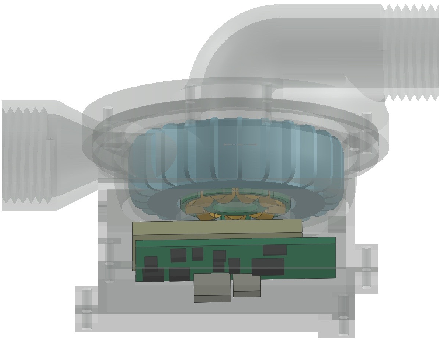
\includegraphics[scale=0.45]{assembled-tethys-sensor.png}
        \caption{\label{étiquette} Assembled Tethys Sensor\cite{IEEEhowto:} The battery (yellow), PBC (green), all encases in a custom enclosure}
    \end{figure}

\end{center}
"\emph{The device is mounted between a water pipe and shower head so
that the generator’s rotor is in line with the water flow. Figure~\ref{étiquette} shows an assembled Tethys device }" \cite{IEEEhowto:}.
The standard approach to waterproofing consumer products is to encase the circuit in resin. Which is not appropriate if we need to reprogram devices after manufacturing. So the good way is to use a waterproof  compartment in order to easily manage potential repairs or upgrades.

The design phase revealed some essential constraints to take into account in order to design the right enclose. They first used a 3D printer that facilitated prototyping of the device, except that its testing showed a large variation in energy harvesting. This is not the desired goal when they try to decouple the device as much as possible from the infrastructure where it is set up.

So they finally use injection molding which is able to satisfy the requirements. There is an initial high cost, but for large manufacturing this cost is insubstantial.\\

\begin{tabular}{|c|c|c|}
\hline
 \cellcolor{gray} & Tethys & Amphiro A1 Basics\cite{amphiro:} \\
\hline
    Price & 36,82 \texteuro & 69,90 \texteuro \\
\hline
\end{tabular}\\

This array compare one existing water sensor device cost with Tethys. We saw that with this design, Tethys is competitive.

\subsection{Infrastructure-Free Networking}
"\emph{Sensors may be used in a mobile setting or in a location
where existing networks inaccessible or unusable}" \cite{IEEEhowto:}. This avoids confronting networks with limited access or the total lack of network infrastructure even if in the case of Tethys it is not likely to happen considering there is always Wifi in student residences.

It is difficult to manually collect sensor data. That's why Tethys "\emph{crowdsources the data-collection task to building residents}" \cite{IEEEhowto:}. As we can see in Figure~\ref{étiquette2} the BLE is in charge to collect data from water sensor such as water flow, temperature to a mobile app acting as a "gateway" in order to further send them to the cloud. There is no need to manage this app for the entire process (background running app). Simply need to get closer from the bathroom location to collect periodically data when the phone have network active.  

\begin{center}
    \begin{figure}[!t]
        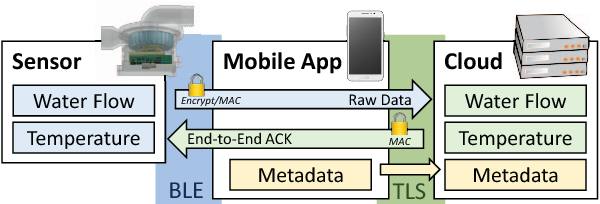
\includegraphics[scale=0.4]{network-design-tethys.png}
        \caption{\label{étiquette2} Network design of Tethys use \cite{IEEEhowto:}}
    \end{figure}
\end{center}
\subsection{Untrusted Gateways}
A strong coupling of the data collection to the devices which the collection can very quickly become a problem for the study envisaged in the document. Several devices of the process can be offline while collecting data. "\emph{Tethys addresses these issues by implementing reliable, delay-tolerant, end-to-end acknowledgement of data from the sensor to the cloud}" \cite{IEEEhowto:}. Actually, each sensor retransmits data when they can, flooding data to each phone-gateway that connects. Tethys allow more conservative policy and less energy consumption. Even if there can be delay tolerant network, this case is managed by the system with an insignificant latency by pre-loading existing data.

"\emph{Tethys requires end-to-end security as well as reliable delivery}" \cite{IEEEhowto:}. Indeed, even if there is no data lost, just the fact that untrusted phones can act as gateway affect privacy and quality of collect data. As we can see in Figure~\ref{étiquette2} Tethys offer this end-to-end security. We'll not develop about the data security strategy and technology used.

\subsection{Data analysis and Evaluation}
\begin{center}
    \begin{figure}[!t]
        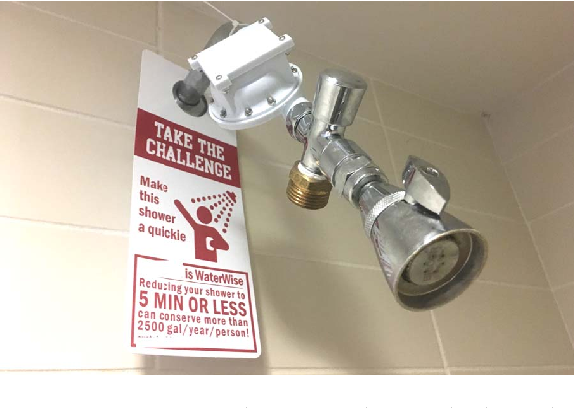
\includegraphics[scale=0.4]{water-message.png}
        \caption{\label{étiquette3} \emph{ Conservation message advocating residents to take shorter showers.} \cite{IEEEhowto:}}
    \end{figure}

\end{center}
In this part, we will see that there is a way to improve data transfer velocity, but also that this study can highlight some showering patterns. They set the following background for the study : 
\begin{itemize}
    \item Analysis of data collected from 3 student residence halls;
    \item Some showers already contained water conservation messages (Figure~\ref{étiquette4});
    \item data collected from 23 sensors during 2 weeks.
\end{itemize}
The purpose for them was to "\emph{measure how their results compare against initial hypotheses about data and water use patterns}" \cite{IEEEhowto:}.

In order to reduce the amount of data to be stored and transmitted, they only collect if there is a change in water flow or temperature. This helps define what they call a compression ratio. For example if we have a compression ratio of 20, it means that for a 200 data points collected normally during a 200 second shower, they remain 10 data points.The better the ratio, the better the compression will be as we can see in Figure~\ref{étiquette4}. Their results show that "\emph{half the toal showers have compression ratios below 20, with a degree of high variance overall}"\cite{IEEEhowto:}. Difference in recorded shower is explained by variations in pressure from specific water usage. More explanations are noticed in the report \cite{IEEEhowto:}.

Concerning showering patterns, they apply some indicators in order to identify correctly showering behavior. The Figure~\ref{étiquette5} highlight the distribution of measured shower lengths. It clears the fact that the median shower length is 7.77 minutes with a huge proportion of showers taking 5 minutes or less. However, The little proportion of consumers taking very long time shower (4\%) need to be target in order to improve water conservation. 
The use of Tethys show that energy harvesting was significantly a succes because with just a single shower is enough to cover mainly energy consumption of the device. 

\begin{center}
    \begin{figure}[!t]
        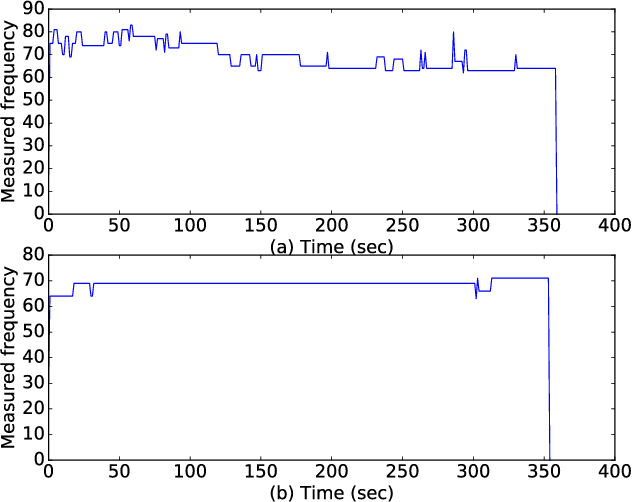
\includegraphics[scale=0.4]{record-shower-comparison.png}
        \caption{\label{étiquette4} \emph{Recorded shower data from a single sensor with delta compression ratio of (a) 7.0 and (b) 35.4} \cite{IEEEhowto:}}
    \end{figure}

\end{center}

\begin{center}
    \begin{figure}[!t]
        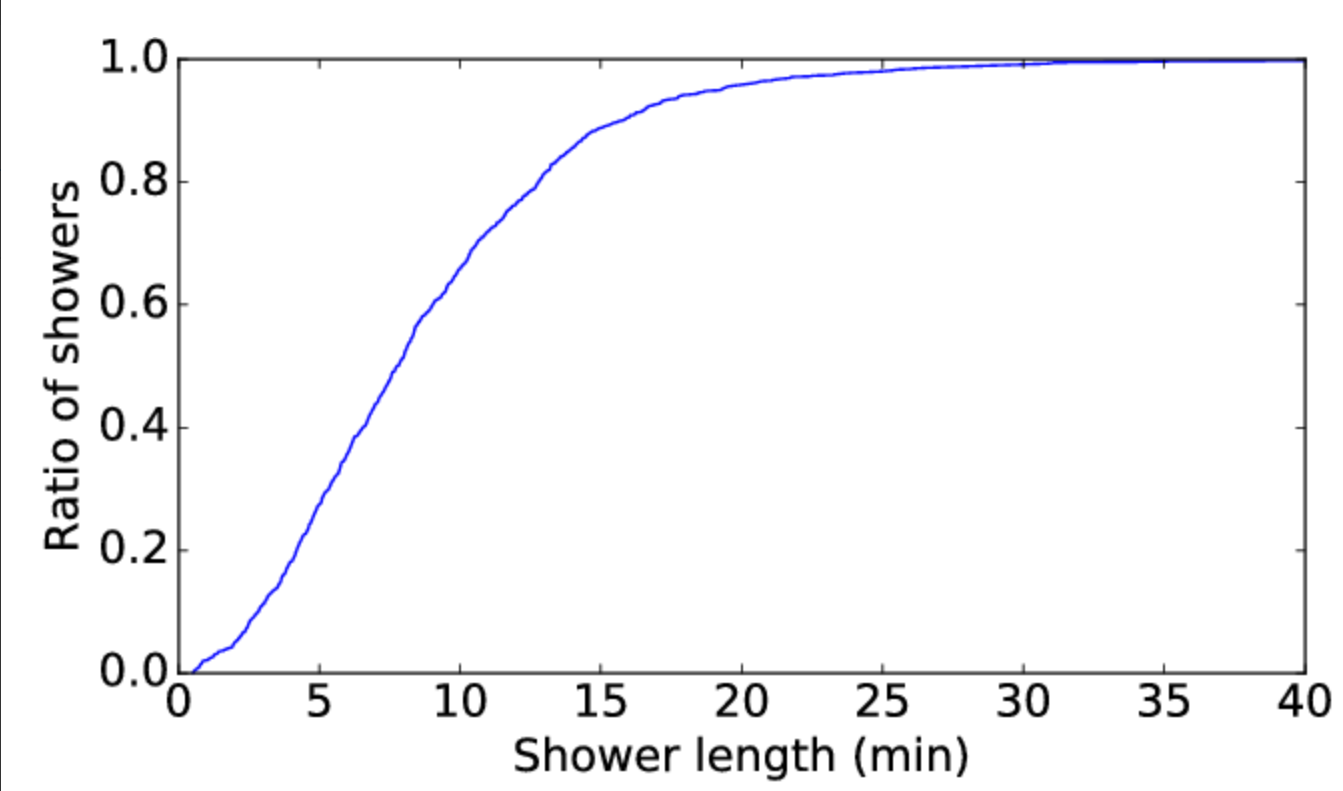
\includegraphics[scale=0.4]{distribution-shower-length.png}
        \caption{\label{étiquette5} \emph{. Cumulative distribution graph of shower lengths} \cite{IEEEhowto:}}
    \end{figure}

\end{center}

\section{Discussion}\label{sec:discussion}
\subsection{Plus/Minus Reviews}


\section{Conclusion}\label{sec:conclusion}

\appendices
\section{Terms definition}
Here we define some terms that need to be explained.
BLE, TLS, Sensor, PBC
\newline



\begin{thebibliography}{2}
\bibitem{IEEEhowto:}
H.~Chiang, J. ~Hong, K. ~Kiningham, L. ~Riliskis, P. ~Levis, and M.~Horowitz, \emph{Tethys: Collecting Sensor Data Without Infrasctructure or Trust}, \hskip 1em plus
  0.5em minus 0.4em\relax 2018 IEEE/ACM Third International Conference on Internet-of-Things Design and Implementation.
\bibitem{amphiro:}
Amphiro. (2018) amphiro. [Online]. Available: http://amphiro.com/
\end{thebibliography}
\end{document}
